% =====================================================================
%  CodeTwin AI -- research paper (IEEE conference format)
%  Group P6, Dept. of CSE (Data Science), TSSM's PVPIT, Pune
%
%  main.tex is generated from main.template.tex by pilot/paper_numbers.py:
%  every number about our study comes from pilot/results/results.json.
%  Edit the template, not main.tex, if you change text around numbers.
% =====================================================================

\documentclass[conference]{IEEEtran}
\IEEEoverridecommandlockouts

\usepackage{cite}
\usepackage{amsmath,amssymb,amsfonts}
\usepackage{algorithm}
\usepackage{algpseudocode}
\usepackage{graphicx}
\usepackage{textcomp}
\usepackage{xcolor}
\usepackage{booktabs}
\usepackage{array}
\usepackage{url}
\usepackage{tikz}
\usetikzlibrary{positioning,arrows.meta,fit}


\makeatletter
\newcommand{\linebreakand}{%
  \end{@IEEEauthorhalign}
  \hfill\mbox{}\par
  \mbox{}\hfill\begin{@IEEEauthorhalign}
}
\makeatother

% Zenodo DOI of the replication package (reserve it on Zenodo before publishing, then replace XXXXXXX).
\newcommand{\replicationdoi}{10.5281/zenodo.XXXXXXX}

\begin{document}

\title{CodeTwin AI: Evidence-Aware, Risk-Calibrated\\
Regression Test Selection with Abstention---\\
A Survey and an Empirical Study on Python Projects}

\author{
\IEEEauthorblockN{Aarya Godbole}
\IEEEauthorblockA{\textit{Dept. of CSE (Data Science)} \\
\textit{TSSM's PVPIT}\\
Pune, India \\
aaryagodbole550@gmail.com}
\and
\IEEEauthorblockN{Suhani Bhati}
\IEEEauthorblockA{\textit{Dept. of CSE (Data Science)} \\
\textit{TSSM's PVPIT}\\
Pune, India \\
bhatisuhani5@gmail.com}
\and
\IEEEauthorblockN{Madhura Suryawanshi}
\IEEEauthorblockA{\textit{Dept. of CSE (Data Science)} \\
\textit{TSSM's PVPIT}\\
Pune, India \\
suryawanshimadhura51@gmail.com}
\linebreakand
\IEEEauthorblockN{Shreya Gole}
\IEEEauthorblockA{\textit{Dept. of CSE (Data Science)} \\
\textit{TSSM's PVPIT}\\
Pune, India \\
shreyakgole@gmail.com}
\and
\IEEEauthorblockN{Dr. T. A. Kamble}
\IEEEauthorblockA{\textit{Dept. of CSE (Data Science)} \\
\textit{TSSM's PVPIT}\\
Pune, India \\
tulsiram17@gmail.com}
}

\maketitle

% =====================================================================

% =====================================================================
\begin{abstract}
Running a full regression test suite after every change is slow, and AI coding assistants increase the number of changes. Regression test selection (RTS) runs only the tests a change may affect, but existing techniques return a fixed subset without stating how much risk remains, and they treat dependencies they cannot resolve as absent. After reviewing twenty-seven related works, we propose CodeTwin AI, which ranks tests with a learned risk model, estimates the residual risk of each selection, calibrates its threshold to a target miss rate with conformal risk control, and abstains to a broader run when the estimated risk is too high. We evaluated a Python prototype on <<N_CHANGES>> changes of <<N_PROJ>> open-source projects with three ground truths: per-test coverage, <<N_MUTANTS>> detected seeded faults, and the published ground truth of NameRTS. Calibration fitted on older commits failed under drift: at a 10\% target it missed affected tests on <<CRC10_MISS>>\% of later changes. With adaptive conformal inference, the observed miss rates were <<ACI5_MISS>>\%, <<ACI10_MISS>>\% and <<ACI20_MISS>>\% for targets of 5\%, 10\% and 20\%. Abstaining when the estimated risk exceeded the target caught <<TR_FLAG_UNSAFE>> of the <<TR_UNSAFE>> changes on which line-coverage selection was unsafe, against <<TL_FLAG_UNSAFE>> for rule-based triggers, and gave <<AR_FILECOV_SAFE>>\% safe changes while saving <<AR_FILECOV_TIME>>\% of test time. The learned ranking did not beat a coverage ranking, and file-level coverage alone was safe on these projects. A selection's residual risk can be stated and held at a chosen level, but only with calibration that adapts over time.
\end{abstract}


\begin{IEEEkeywords}
abstention, adaptive conformal inference, change impact analysis, conformal risk control, mutation testing, regression test selection
\end{IEEEkeywords}


% =====================================================================
\section{Introduction}\label{sec:intro}
% =====================================================================

% P1 -- Context and motivation
Regression testing checks whether a code change breaks previously working behaviour~\cite{yoo2012survey}. As suites grow, rerunning every test after each change raises execution costs and strains continuous integration (CI) at scale~\cite{elbaum2014ci,memon2017taming}. Developers must balance these costs against the risk of omitting tests that a change affects. AI-assisted development sharpens this trade-off, because patches may arrive faster than developers can inspect their effects. A preprint evaluating an agent on SWE-bench Verified reported regressions with a locally hosted open-weight model, and found that information about potentially affected tests reduced such failures~\cite{alonso2026tdad}. This is preliminary evidence rather than a general conclusion about AI-generated code, but it shows why identifying the relevant tests matters. Regression test selection (RTS) reruns only a subset of the suite, and the value of that subset depends on how well the risk of missing affected tests is understood.

% P2 -- Existing approaches, limitations, and research gaps
RTS selects tests using dependencies between changed code and tests; a selection is \emph{safe} if it retains every potentially affected test~\cite{legunsen2016static}. Gligoric et al.\ introduced Ekstazi, which recorded the files each test accessed and reran a test only when one of them changed~\cite{gligoric2015ekstazi}. Liu et al.\ reasoned about semantics-modifying changes so that tests affected only by certain such changes were not rerun~\cite{liu2023finerts}, and JcgEks combined dynamic file dependencies with static method call graphs~\cite{zhang2024jcgeks}. These techniques target Java. Python poses additional challenges because imports can execute code and dynamic features obscure call targets. NameRTS used name matching and run-time probes for reflection, and retained every affected test file on 99.6\% of 500 commits across ten projects~\cite{wang2026namerts}. Predictive test selection (PTS), by contrast, learned from historical outcomes which tests were likely to fail~\cite{machalica2019pts}.

In the work we reviewed, three gaps remain. First, good average performance does not itself provide a calibrated assessment of residual risk for a particular selection; PTS thresholds estimated from historical samples should not be read as guarantees for individual commits~\cite{machalica2019pts}. Second, dependency evidence may be incomplete without exposing why: NameRTS documents limitations involving \texttt{eval}, library code, and an affected test reached through an external-library callback~\cite{wang2026namerts}. Third, broader testing is not necessarily triggered by weak evidence for the current change: NameRTS selects all tests when a registry decorator changes~\cite{wang2026namerts}, while PTS may rely on periodic full-suite runs~\cite{machalica2019pts}. Conformal risk control can bound the expected value of a monotone loss, such as miss rate, under assumptions including exchangeability~\cite{angelopoulos2024crc}; related work studies conformal abstention for language-model hallucinations~\cite{yadkori2024abstention} and conformal methods for test prioritisation in CI~\cite{altinisik2026conformal}. To our knowledge, none of the reviewed techniques combines risk calibration, visible dependency limitations and uncertainty-triggered fallback in RTS.

% P3 -- Research question and methodology
This paper asks: \emph{for software repositories, evaluated first on Python projects, can evidence-aware test selection with calibrated abstention keep the miss rate at a chosen target while running substantially fewer tests than the full suite, and does it flag the changes on which conventional selection fails?} We follow an engineering-research method: we design and implement CodeTwin AI, a Python prototype, and compare it with established baselines on the commit histories of open-source projects. Changes are processed in time order, so every decision about a change uses only that project's earlier information.

% Objectives (from the project synopsis)
The project has five objectives: (O1)~an evidence graph that records how files, functions, tests and other repositories are connected and how each link was found; (O2)~risk-ranked test selection within a time budget; (O3)~an estimate of the residual risk of a selection, calibrated to a target miss rate, with abstention when the evidence is insufficient; (O4)~integration into the developer workflow and AI coding agents; and (O5)~an evaluation against established baselines on public projects. This paper implements the evidence collection of O1 and the selection, calibration and abstention of O2 and O3 for single Python repositories, and evaluates them as O5. The evidence store of O1 and a first version of the O4 interfaces have since been implemented in the CodeTwin AI tool (release 0.1.0) but are not evaluated here; cross-repository links are designed but not yet implemented.

% P4 -- Contributions and principal findings
We make four contributions.
\begin{itemize}
    \item A survey of twenty-seven works on test selection, coverage, call graphs, calibrated prediction and testing support for AI agents, and the gap between efficient selection and a stated residual risk (Sections~\ref{sec:related} and~\ref{sec:gap}).
    \item CodeTwin AI, which keeps unresolved dependencies as uncertainty, ranks tests by learned risk per second, estimates the residual risk $r(c)$ of each selection, calibrates its threshold with conformal risk control that adapts to drift, and abstains to a broader run when the risk is too high (Sections~\ref{sec:approach} and~\ref{sec:impl}).
    \item An evaluation on <<N_CHANGES>> changes of <<N_PROJ>> Python projects with three ground truths (per-test coverage, <<N_MUTANTS>> seeded faults and, on <<N_NRTS_PROJ>> projects, the published ground truth and selections of NameRTS), against ten baselines, including the published NameRTS selections (Sections~\ref{sec:setup} and~\ref{sec:results}). Calibration fitted on older commits failed under drift; adaptive calibration kept the observed miss rate at or below the target on the history projects and close to it on the shorter NameRTS histories, and risk-based abstention detected most unsafe changes with far fewer false alarms than rule-based triggers.
    \item A replication package archived on Zenodo: scripts, the GitHub Actions workflows, the collected data of every change and every reported number.
\end{itemize}

% P5 -- Paper organisation
Section~\ref{sec:background} introduces key concepts and a motivating example. Section~\ref{sec:related} reviews prior work and Section~\ref{sec:gap} states the research gap. Sections~\ref{sec:approach} and~\ref{sec:impl} present the approach and its implementation, Sections~\ref{sec:setup} and~\ref{sec:results} the evaluation, Section~\ref{sec:discussion} the implications, Section~\ref{sec:threats} the threats to validity and Section~\ref{sec:conclusion} the conclusions.

% =====================================================================
\section{Background and Motivating Example}\label{sec:background}
% =====================================================================
\subsection{Key Concepts}
When code changes, \textit{regression test selection} (RTS) reruns only some of the tests instead of all of them. A selection is \textit{safe} if it skips no test that the change could make fail~\cite{yoo2012survey}. \textit{Test prioritisation} does something different: it puts the tests in a better order, but it never drops any~\cite{yoo2012survey}. To decide which tests matter, tools use \textit{change impact analysis}, which finds the functions, files, tests and repositories a change can touch. This analysis can be \textit{static}, reading the code without running it, or \textit{dynamic}, watching the code run. Static analysis cannot follow calls such as \texttt{getattr} or \texttt{importlib}, while dynamic analysis only sees the paths that were actually executed. \textit{Per-test code coverage} records which lines each test runs, so we can tell which tests cover a change and which changed lines no test covers.

A good tool should also say how risky its choice is. The \textit{miss rate} is the share of changes where a test that should have run was left out. A risk estimate is \textit{calibrated} if the predicted probability matches how often the event really happens; for example, changes labelled 5\% risky should be missed about 5\% of the time. \textit{Conformal risk control} uses held-out data to pick a threshold that keeps the expected miss rate below a chosen target~\cite{angelopoulos2024crc}. Its guarantee assumes that calibration changes and future changes are \textit{exchangeable}, which commits ordered in time need not be; \textit{adaptive conformal inference} instead adjusts the target level online after each observed error, so that the long-run error rate tracks the target even when the data drift~\cite{gibbs2021aci}. Finally, \textit{abstention} means the system admits it is unsure when its evidence is weak~\cite{yadkori2024abstention}. In our case, it then recommends running more tests instead of a small set. Lastly, \textit{mutation testing} seeds small artificial faults, called mutants, into a program; a test \textit{detects} (kills) a mutant if it fails on it, and mutant detection is a widely used and validated stand-in for detecting real faults~\cite{jia2011mutation,just2014mutants}.
\subsection{Motivating Example}
Consider the case in Fig.~\ref{fig:example}. A pull request renames the field \texttt{price} of \texttt{orders.Order} in a shared library, and all of the library's tests pass. The change has four dependants, and each is known in a different way: \texttt{billing.total()} is a static caller in the same repository; \texttt{vendor\_portal/pricing.py} is a consumer in another repository, declared in an OpenAPI contract; \texttt{customer\_app/cart.py} is a consumer in another repository that is seen only at run time and has no tests; and \texttt{plugins.load()} uses \texttt{getattr}, so its target cannot be resolved statically. In the figure, line style shows how each link was found. A conventional tool links the change to two tests, \texttt{test\_billing.py} and \texttt{test\_pricing.py}, and reports it as ``verified''. What it misses is the untested consumer, which no selected test can catch, and the unresolved call, which it treats as unaffected instead of reporting. CodeTwin AI reports instead the two blind spots, the remaining risk, which these two blind spots would push above a 5\% target, and a recommendation to run more tests. Passing tests in the changed repository therefore do not show that a change is safe. The next sections describe how CodeTwin AI builds this evidence and turns it into such a recommendation.

\begin{figure}[t]
\centerline{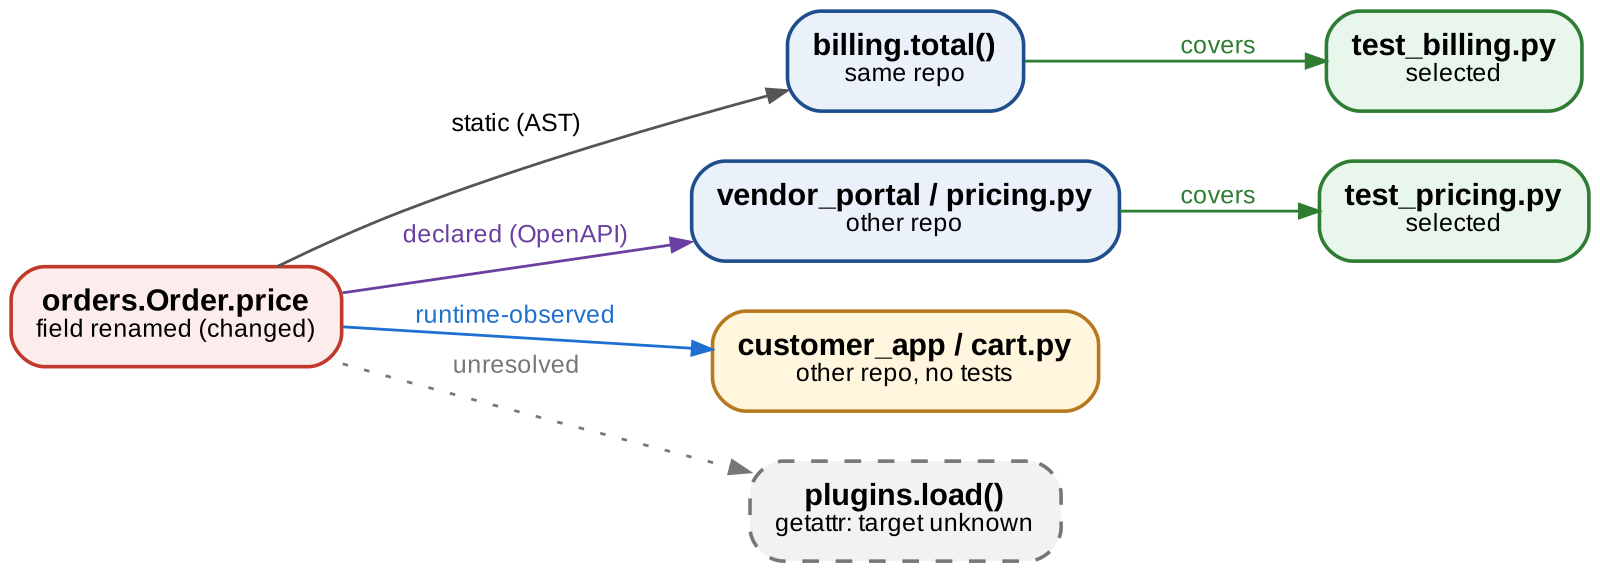
\includegraphics[width=\columnwidth]{figures/example.png}}
\caption{Impact map for renaming \texttt{orders.Order.price} (red). Line style shows how each link was found: static analysis (AST), a declared OpenAPI contract, runtime observation, or unresolved (dotted). Green nodes are the selected tests, the orange node is a consumer with no tests, and the dashed node, \texttt{plugins.load()}, uses \texttt{getattr}, so its target is unknown.}
\label{fig:example}
\end{figure}

% =====================================================================
\section{Related Work}\label{sec:related}
% =====================================================================
We searched Google Scholar, arXiv, the ACM Digital Library and IEEE Xplore for work on regression test selection, change impact analysis, static and dynamic dependency analysis, test coverage, learned test selection, conformal prediction and abstention, and testing support for AI coding agents. Venues of interest were ISSTA, ASE, ICSE, FSE and ICLR. We covered mainly 2015--2026, adding earlier foundational studies where relevant. We kept 27 works that are foundational or closest to our problem, and we did not aim for exhaustive coverage. We organise them into six themes: foundations, precise and hybrid selection, coverage and change structure, Python selection, learned selection and test generation, and calibration, abstention and AI coding agents. Table~\ref{tab:survey} summarises the reviewed works.


\subsection{Foundations of Regression Test Selection}
Yoo and Harman~\cite{yoo2012survey} separate test-suite minimisation, regression test selection (RTS) and test-case prioritisation, and RTS reruns only the tests that a change may affect. Rothermel and Harrold~\cite{rothermel1996analyzing} proposed a framework for comparing selection techniques; its criteria include inclusiveness (a fully inclusive technique is safe), precision, efficiency and generality. Ekstazi records the files that each test uses at run time and reruns a test when one of them changes; on 615 revisions of 32 projects it reduced end-to-end testing time by 32\% on average compared with running all tests~\cite{gligoric2015ekstazi}. Legunsen et al.\ studied static selection on 985 revisions of 22 projects and found that a class-level technique performed comparably to Ekstazi but was sometimes unsafe, while a method-level technique performed poorly~\cite{legunsen2016static}. STARTS is a Maven tool for static class-level selection that needs no instrumentation or runtime information; the authors report that it selected on average 35.2\% of tests, with an end-to-end time of 81.0\% of running all tests~\cite{legunsen2017starts}. unlike Ekstazi, the static technique does not need a test run to collect dependencies. These studies report safety and savings as aggregates over revisions, not a calibrated estimate of the risk left by the selection for one change. The kind of dependency evidence therefore decides both the savings and the conditions under which tests can be omitted safely.

\subsection{Precise and Hybrid Selection}
File-level dependencies keep analysis cheap but can select tests that a change cannot affect; Ekstazi, for example, selected more tests than the method-level tool FaultTracer on the six projects where both ran, yet had a much lower end-to-end time~\cite{gligoric2015ekstazi}. Liu et al.\ inspected changes in five projects and found that some semantics-modifying changes need not trigger tests that they alone affect, and built FineEkstazi and FineSTARTS on this finding. On 1,150 versions of 23 projects, the variants selected on average 41.7\% and 31.8\% fewer test classes and took 33.7\% and 28.7\% less time than Ekstazi and STARTS, respectively, with no new safety violations reported by RTSCheck~\cite{liu2023finerts}. JcgEks combines Ekstazi's dynamic file dependencies with static method call graphs and is designed to handle callbacks from external libraries safely. On 1,000 revisions of 20 projects, it selected 29.0\% fewer test classes and took 30.9\% less end-to-end time than Ekstazi without missing any test class in the authors' safety check; compared with FineEkstazi it had a similar end-to-end time and number of selected test classes, while FineEkstazi was confirmed to miss test classes~\cite{zhang2024jcgeks}. HyRTS combines method-level and file-level analysis; on 2,707 revisions of 32 projects it outperformed file-level selection in selected test ratio and offline testing time~\cite{zhang2018hyrts}. The applicability and guarantees of these techniques depend on their dependency models, language support and treatment of unresolved dependencies. In the evaluations we checked, safety and savings are aggregate results, not a per-change risk estimate, which is the gap that CodeTwin AI addresses.

\subsection{Coverage and Change Structure}
Prioritisation orders tests instead of removing them. Rothermel et al.\ ordered tests by total coverage, additional coverage or estimated fault-revealing ability, and compared the rate of fault detection with untreated, random and optimal orders~\cite{rothermel2001prioritizing}. Coverage itself is costly to refresh after every change. iJaCoCo, built on Ekstazi and JaCoCo, executes a minimal subset of tests to update only the coverage affected by a change. On 1,122 versions of 22 repositories it sped up end-to-end coverage analysis by 1.86$\times$ on average and up to 8.20$\times$ compared with JaCoCo; it was faster on 17 of the 22 repositories and selected 47.34\% of test classes, against 20.63\% for Ekstazi~\cite{wang2024ijacoco}. Altiero et al.\ apply tree kernels to abstract syntax trees to quantify structural change and prioritise tests; on five real-world Java projects, using 100 fault-injected variants per version pair (over 5,000 scenarios), they report better prioritisation effectiveness than well-known techniques with typically negligible overhead~\cite{altiero2024treekernel}. Ivankovi\'c et al.\ describe coverage at Google, applied to changesets and code review, with five years of adoption data and 512 survey responses from 3,000 developers~\cite{ivankovic2019coverage}; this is evidence from industrial practice, not a controlled experiment. Executing a line does not show that a test detects a fault, and none of these works estimates the risk of a selection. Coverage has a scope and a collection time, and structural change is a complementary signal; both matter when CodeTwin AI uses coverage from the previous commit together with structural change features.

\subsection{Selection for Python}
Python complicates dependency analysis because modules run code when they are imported and many call targets are known only at run time. PyCG builds static call graphs for Python by tracking assignments across modules; on a micro-benchmark of small programs and a set of real-world packages it reached about 99.2\% precision but only about 69.9\% recall~\cite{salis2021pycg}. Roughly three in ten real call edges were therefore missing from the graph, and a selection technique built on such a graph would treat them as absent dependencies. NameRTS avoids call-graph construction: it models a program as a bipartite graph of code elements and names, and selects a test when a modified element is reachable from a name that the test uses~\cite{wang2026namerts}. On a new dataset of 500 commits from ten projects it skipped 69.9\% of the test files on average, reduced end-to-end testing time by 45.6\%, and selected all affected tests on 99.6\% of commits, whereas a file-level baseline was safe on only 76.6\%. NameRTS is conservative by design, but its answer is still a yes-or-no subset: it does not state how much risk remains for a particular commit, and its rare misses are not reported to the developer when they happen. Coverage-based selection has also been built for Python. Kauhanen et al.\ integrated a coverage-based selection tool into continuous integration and evaluated it with mutation testing on three open-source projects; selected subsets missed 0--2\% of faults at file granularity but 16--24\% at line granularity~\cite{kauhanen2021python}. For prioritisation, pytest-ranking reorders pytest suites; on 4,308 GitHub Actions builds of 14 Python projects it revealed failures earlier than the default and random orders with low overhead~\cite{cheng2025pytestranking}. In dynamic languages a sizeable share of real dependencies is invisible to static analysis, so a selection technique should expose this blind spot rather than hide it.

\subsection{Learned Selection and Test Generation}
Learned selection replaces explicit dependencies with models trained on past test outcomes. Machalica et al.\ trained a model on historical results at Meta to predict which tests a code change is likely to break; in production it reported more than 95\% of individual test failures and more than 99.9\% of faulty changes to developers while halving the infrastructure cost of testing~\cite{machalica2019pts}. These figures are aggregates over many changes: the selection threshold is set from historical samples, and a developer receives no statement about the risk left for the change in front of them. Bertolino et al.\ compared ten machine-learning algorithms for regression testing in continuous integration, contrasting learning-to-rank with ranking-to-learn (reinforcement learning) on subjects from the Apache Commons project, and analysed how properties of the code and of the test process decide which strategy fits best~\cite{bertolino2020learning}. Language models have also been used to write tests. Foster et al.\ described ACH at Meta, which generates mutants for one concern, such as privacy, and then writes tests that catch them; applied to 10,795 Android Kotlin classes on seven platforms it produced 9,095 mutants and 571 privacy-hardening tests, and engineers accepted 73\% of the tests offered in test-a-thons~\cite{foster2025ach}. Learning therefore helps to rank and to generate tests, but the confidence it reports is aggregate, and language-model output became useful only after it was checked by execution and by engineers.

\subsection{Calibration, Abstention and AI Coding Agents}
Conformal methods give distribution-free guarantees from a held-out calibration set; Angelopoulos and Bates introduce them for practitioners~\cite{angelopoulos2023gentle}. Conformal risk control extends conformal prediction to bound the expected value of any monotone loss, such as a false-negative rate, at a chosen level under exchangeability~\cite{angelopoulos2024crc}. Abbasi Yadkori et al.\ use conformal prediction to decide when a language model should abstain; their method kept the hallucination rate within its bound on two question-answering datasets and abstained far less often than log-probability baselines on long answers~\cite{yadkori2024abstention}. In software engineering, Shahini et al.\ applied conformal prediction to two just-in-time defect predictors on the Qt and OpenStack datasets; at 95\% confidence the guarantee held for only 27\% and 9\% of their predictions, while the method filtered out most of their false positives and false negatives~\cite{shahini2024jitcp}. Closest to testing, Alt{\i}n{\i}{\c{s}}{\i}k combined history-based prioritisation in continuous integration with adaptive conformal calibration; on 273 failure-bearing jobs of four Java projects, calibration reduced the candidate set from about 32\% to about 26\% of the tests while keeping about 91\% of the failing tests~\cite{altinisik2026conformal}. That work orders tests; it does not bound the risk left by a selection for each change.

AI coding agents make this gap practical. SWE-bench collects 2,294 real issues from 12 Python repositories; when it was introduced, the best model resolved 1.96\% of them~\cite{jimenez2024swebench}. Venkatesh et al.\ evaluated 24 language models and found that static tools such as PyCG still built more complete and sound call graphs~\cite{venkatesh2025llmcg}, so model output cannot replace analysis. TDAD gives an agent a static code-to-test map before it commits a patch; on SWE-bench Verified with open-weight models it reduced the regression rate from 6.08\% to 1.82\%~\cite{alonso2026tdad}. The map, however, carries no calibrated confidence, and the agent is never told to stop. Calibration and abstention methods with guarantees exist, and agents need test-selection support, but in our search the two have not been combined.

\begin{table*}[t]
\caption{Summary of the Reviewed Literature}
\label{tab:survey}
\centering
\footnotesize
\renewcommand{\arraystretch}{1.15}
\begin{tabular}{@{}>{\raggedright\arraybackslash}p{0.06\textwidth}>{\raggedright\arraybackslash}p{0.22\textwidth}>{\raggedright\arraybackslash}p{0.19\textwidth}>{\raggedright\arraybackslash}p{0.22\textwidth}>{\raggedright\arraybackslash}p{0.21\textwidth}@{}}
\toprule
\textbf{Work} & \textbf{Approach} & \textbf{Evaluation} & \textbf{Key finding} & \textbf{Limitation for our problem} \\
\midrule
\cite{yoo2012survey} & Survey of minimisation, selection, prioritisation & Literature survey & Separates three testing problems & No calibrated risk estimate \\
\cite{rothermel1996analyzing} & Safety and precision criteria & Analytical framework & Basis for comparing RTS techniques & Criteria are not per-change risk \\
\cite{gligoric2015ekstazi} & Dynamic file-dependency selection & 615 revisions, 32 projects & 32\% less end-to-end time & No per-change residual-risk estimate \\
\cite{legunsen2016static} & Static class- and method-level selection & 985 revisions, 22 projects & Class-level comparable to Ekstazi & Class-level sometimes unsafe \\
\cite{legunsen2017starts} & Static class-level selection tool & Tool demonstration & 35.2\% of tests; 81.0\% of full time & No per-change risk estimate \\
\cite{liu2023finerts} & Semantics-modifying change reasoning & 1,150 versions, 23 projects & 41.7\%/31.8\% fewer tests & Fixed subset; no risk estimate \\
\cite{zhang2024jcgeks} & Dynamic files plus static call graphs & 1,000 revisions, 20 projects & 29.0\% fewer classes, 30.9\% less time vs.\ Ekstazi & Fixed subset; no risk estimate \\
\cite{zhang2018hyrts} & Hybrid method- and file-level analysis & 2,707 revisions, 32 projects & Beat file-level selection & Fixed subset; no risk estimate \\
\cite{rothermel2001prioritizing} & Coverage- and fault-based test ordering & Experiments on program test suites & All orders improved fault-detection rate & Orders tests; does not select \\
\cite{wang2024ijacoco} & Incremental coverage updates & 1,122 versions, 22 repositories & 1.87$\times$ average speedup vs.\ JaCoCo & Coverage is not fault detection \\
\cite{altiero2024treekernel} & AST tree-kernel prioritisation & Five Java projects; 5,000+ scenarios & Better ordering, small overhead & Orders tests; removes none \\
\cite{ivankovic2019coverage} & Industrial coverage at changeset level & Five-year data; 512 survey responses & Coverage used in code review & Practice study; not fault-detection proof \\
\cite{salis2021pycg} & Static Python call graphs & Micro- and macro-benchmarks & ${\sim}$99.2\% precision, ${\sim}$69.9\% recall & Missing edges silently absent \\
\cite{wang2026namerts} & Name-based Python selection & 500 commits, 10 projects & 69.9\% files skipped; safe on 99.6\% & Binary; misses not reported \\
\cite{kauhanen2021python} & Coverage-based Python selection in CI & Mutation testing, 3 projects & 0--2\% faults missed (file), 16--24\% (line) & Fixed granularity; no risk estimate \\
\cite{cheng2025pytestranking} & Test prioritisation plugin for pytest & 4,308 CI builds, 14 projects & Failures found earlier than default order & Orders tests; removes none \\
\cite{machalica2019pts} & Learned selection from history & Meta production data & $>$95\% failures found at half the cost & Aggregate confidence only \\
\cite{bertolino2020learning} & Ten ML ranking algorithms in CI & Apache Commons subjects & Context decides best strategy & Orders tests; no risk estimate \\
\cite{foster2025ach} & LLM mutation-guided test generation & 10,795 Android Kotlin classes & 73\% of tests accepted & Not aimed at selection risk \\
\cite{angelopoulos2023gentle} & Conformal prediction tutorial & Methods and examples & Distribution-free coverage guarantees & Not applied to testing \\
\cite{angelopoulos2024crc} & Conformal risk control & Vision and NLP tasks & Bounds expected monotone loss & Not applied to test selection \\
\cite{yadkori2024abstention} & Conformal abstention for LLMs & Two QA datasets & Bounded hallucination rate & Not applied to code \\
\cite{shahini2024jitcp} & Conformal just-in-time defect prediction & Qt and OpenStack datasets & Guarantee for 27\%/9\% of predictions & Predicts defects; does not select tests \\
\cite{altinisik2026conformal} & CI prioritisation with conformal calibration & 273 jobs, 4 Java projects & ${\sim}$91\% failing tests at ${\sim}$26\% of tests & Orders tests; no per-change risk \\
\cite{jimenez2024swebench} & Benchmark of real GitHub issues & 2,294 issues, 12 repositories & Best model resolved 1.96\% & Measures fixes, not regressions \\
\cite{venkatesh2025llmcg} & LLMs for types and call graphs & 24 LLMs, new benchmarks & PyCG beats LLMs on call graphs & LLM edges need verification \\
\cite{alonso2026tdad} & Code-to-test map for agents & SWE-bench Verified & Regressions 6.08\% $\to$ 1.82\% & Uncalibrated; agent never stops \\
\bottomrule
\end{tabular}
\end{table*}


\subsection{Summary and Research Gap}\label{sec:gap}
Table~\ref{tab:gap} compares the closest work with CodeTwin AI; its columns give the language, whether more than one repository is supported, whether a risk estimate is given for a single change, whether calibrated abstention is applied, and whether blind spots are reported. Four observations follow from the review in Sections~III-A to III-F.
\begin{enumerate}
\item Techniques report savings and safety as averages over many commits, for example safe selection on 99.6\% of commits for NameRTS~\cite{wang2026namerts}, but none reports how much risk remains for one particular change.
\item Calls that static analysis cannot resolve, such as those made through \texttt{getattr}, are handled silently instead of being reported to the developer~\cite{salis2021pycg,zhang2024jcgeks}.
\item Calibration and abstention with statistical guarantees exist~\cite{angelopoulos2024crc,yadkori2024abstention}, and conformal calibration has been used to order tests in continuous integration~\cite{altinisik2026conformal}, but not to select tests for one change with a stated risk and an option to abstain.
\item Most techniques support one language and one repository: the semantics-aware and hybrid selectors target Java~\cite{liu2023finerts,zhang2024jcgeks}, NameRTS targets Python~\cite{wang2026namerts}, and none of the reviewed techniques follows dependants into other repositories.
\end{enumerate}
In our search we did not find a technique that combines a per-change residual-risk estimate, calibration of that estimate against a target miss rate, abstention when the evidence is weak, and an explicit report of what the analysis cannot see; our search was limited, and we do not claim that no such work exists.
\begin{table}[t]
\caption{Comparison of the Closest Work With CodeTwin AI}
\label{tab:gap}
\centering
\footnotesize
\setlength{\tabcolsep}{2.5pt}
\begin{tabular}{@{}lccccc@{}}
\toprule
\textbf{Work} & \textbf{Lang.} & \textbf{X-repo} & \textbf{Risk} & \textbf{Abstain} & \textbf{Blind spots} \\
\midrule
NameRTS & Python & No & No & No & No \\
Predictive Test Sel. & Any & No & Aggregate & No & No \\
Conformal CI ranking & Java & No & No & No & No \\
TDAD & Python & No & Score & No & No \\
\textbf{CodeTwin AI} & Python & Design & Yes & Yes & Yes \\
\bottomrule
\end{tabular}
\end{table}

% =====================================================================
\section{Proposed Approach: CodeTwin AI}\label{sec:approach}
% =====================================================================

\subsection{Problem Formulation}
Let $c$ be a commit that changes some source files of a project whose test suite is $T$. CodeTwin AI selects at the level of test files. The run time $t(i)$ of a test file $i\in T$ is measured on the previous commit; a test file that did not exist before receives the median run time. Let $A(c)\subseteq T$ be the test files that are truly affected by $c$ (defined in Section~\ref{sec:setup}), and let $F(c)\subseteq T$ be the test files that $c$ adds or modifies. Test files in $F(c)$ are always run. For each commit the system returns a subset $S(c)$ with $F(c)\subseteq S(c)$ and a decision, \textsc{Proceed} or \textsc{Abstain}, where abstaining means that a broader set of tests is run (the full suite, or a broader evidence-based selection). A commit is \emph{missed} if $A(c)\nsubseteq S(c)$.

The framework has two operating modes. In \emph{budget mode} the developer fixes a time budget $B$ and the selection must satisfy
\begin{equation}
\textstyle\sum_{i\in S(c)} t(i) \le B . \label{eq:budget}
\end{equation}
In \emph{calibrated mode} the developer fixes a target miss rate $\alpha$, and the selection must keep the expected miss rate over future commits at or below that target:
\begin{equation}
\mathbb{E}\big[\,\mathbf{1}\{A(c)\nsubseteq S(c)\}\,\big] \le \alpha . \label{eq:risk}
\end{equation}
We call the probability that a selection misses an affected test its \emph{residual risk} and write $r(c)$ for its estimate for one change (Section~\ref{sec:risk}). Calibrated mode bounds the miss rate over changes; abstention handles single changes whose estimated risk is too high.

We make three assumptions explicit. First, selection works on whole test files, the unit at which pytest reports run times and at which most Python projects organise their tests; selecting individual test functions would use the same evidence but let the start-up cost of the test runner dominate. Second, tests are assumed to be deterministic: flaky tests, which can pass and fail on the same code~\cite{parry2022flaky}, are not modelled. Third, the decision for $c$ may use only information that is available before the tests of $c$ run, namely the diff and the static facts of $c$ and the dynamic evidence (coverage and run times) recorded on the previous commit. Because budgets are usually stated relative to the full suite, we write $B=b\cdot\sum_{i\in T}t(i)$ with $b\in(0,1]$ and report results for $b\in\{0.10,0.25,0.50\}$.

\subsection{Architecture}
Fig.~\ref{fig:arch} shows the four layers of CodeTwin AI. \emph{Layer~1} collects evidence about a change: the changed lines from the git diff, imports and dynamic-call markers from language adapters (the Python \texttt{ast} module first, tree-sitter parsers for further languages), per-test coverage and run times from the test runner, declared dependencies from package manifests and API contracts, and, optionally, suggestions from a locally run language model. \emph{Layer~2} stores every finding as an evidence record and builds a typed dependency graph. \emph{Layer~3} ranks and selects tests, estimates the residual risk of the selection and decides whether to abstain. \emph{Layer~4} delivers the result to developers in a VS Code extension and as a pull-request check, and to AI coding agents through a Model Context Protocol (MCP) server. The prototype evaluated in this paper implements the Python parts of Layers~1 and~3 (Section~\ref{sec:impl}); the evidence store, the language-model suggestions and the Layer~4 interfaces belong to the design and are not evaluated here.

Four design choices shape the architecture. First, the analysis is \emph{local first}: it runs on the developer's machine or on the continuous-integration runner, and no code leaves it unless the optional language model is enabled. Second, \emph{transparent models come first}: logistic regression or gradient boosting rather than deep learning, so that every score can be traced to its features. Third, each language needs only an \emph{adapter}, consisting of a parser, a test runner and a coverage collector that write evidence in a common format; everything above Layer~1 is shared, which makes the framework language-independent although Python is implemented first. Fourth, SQLite and NetworkX replace a graph database, which is sufficient for repositories of the sizes we target.

\begin{figure*}[t]
\centerline{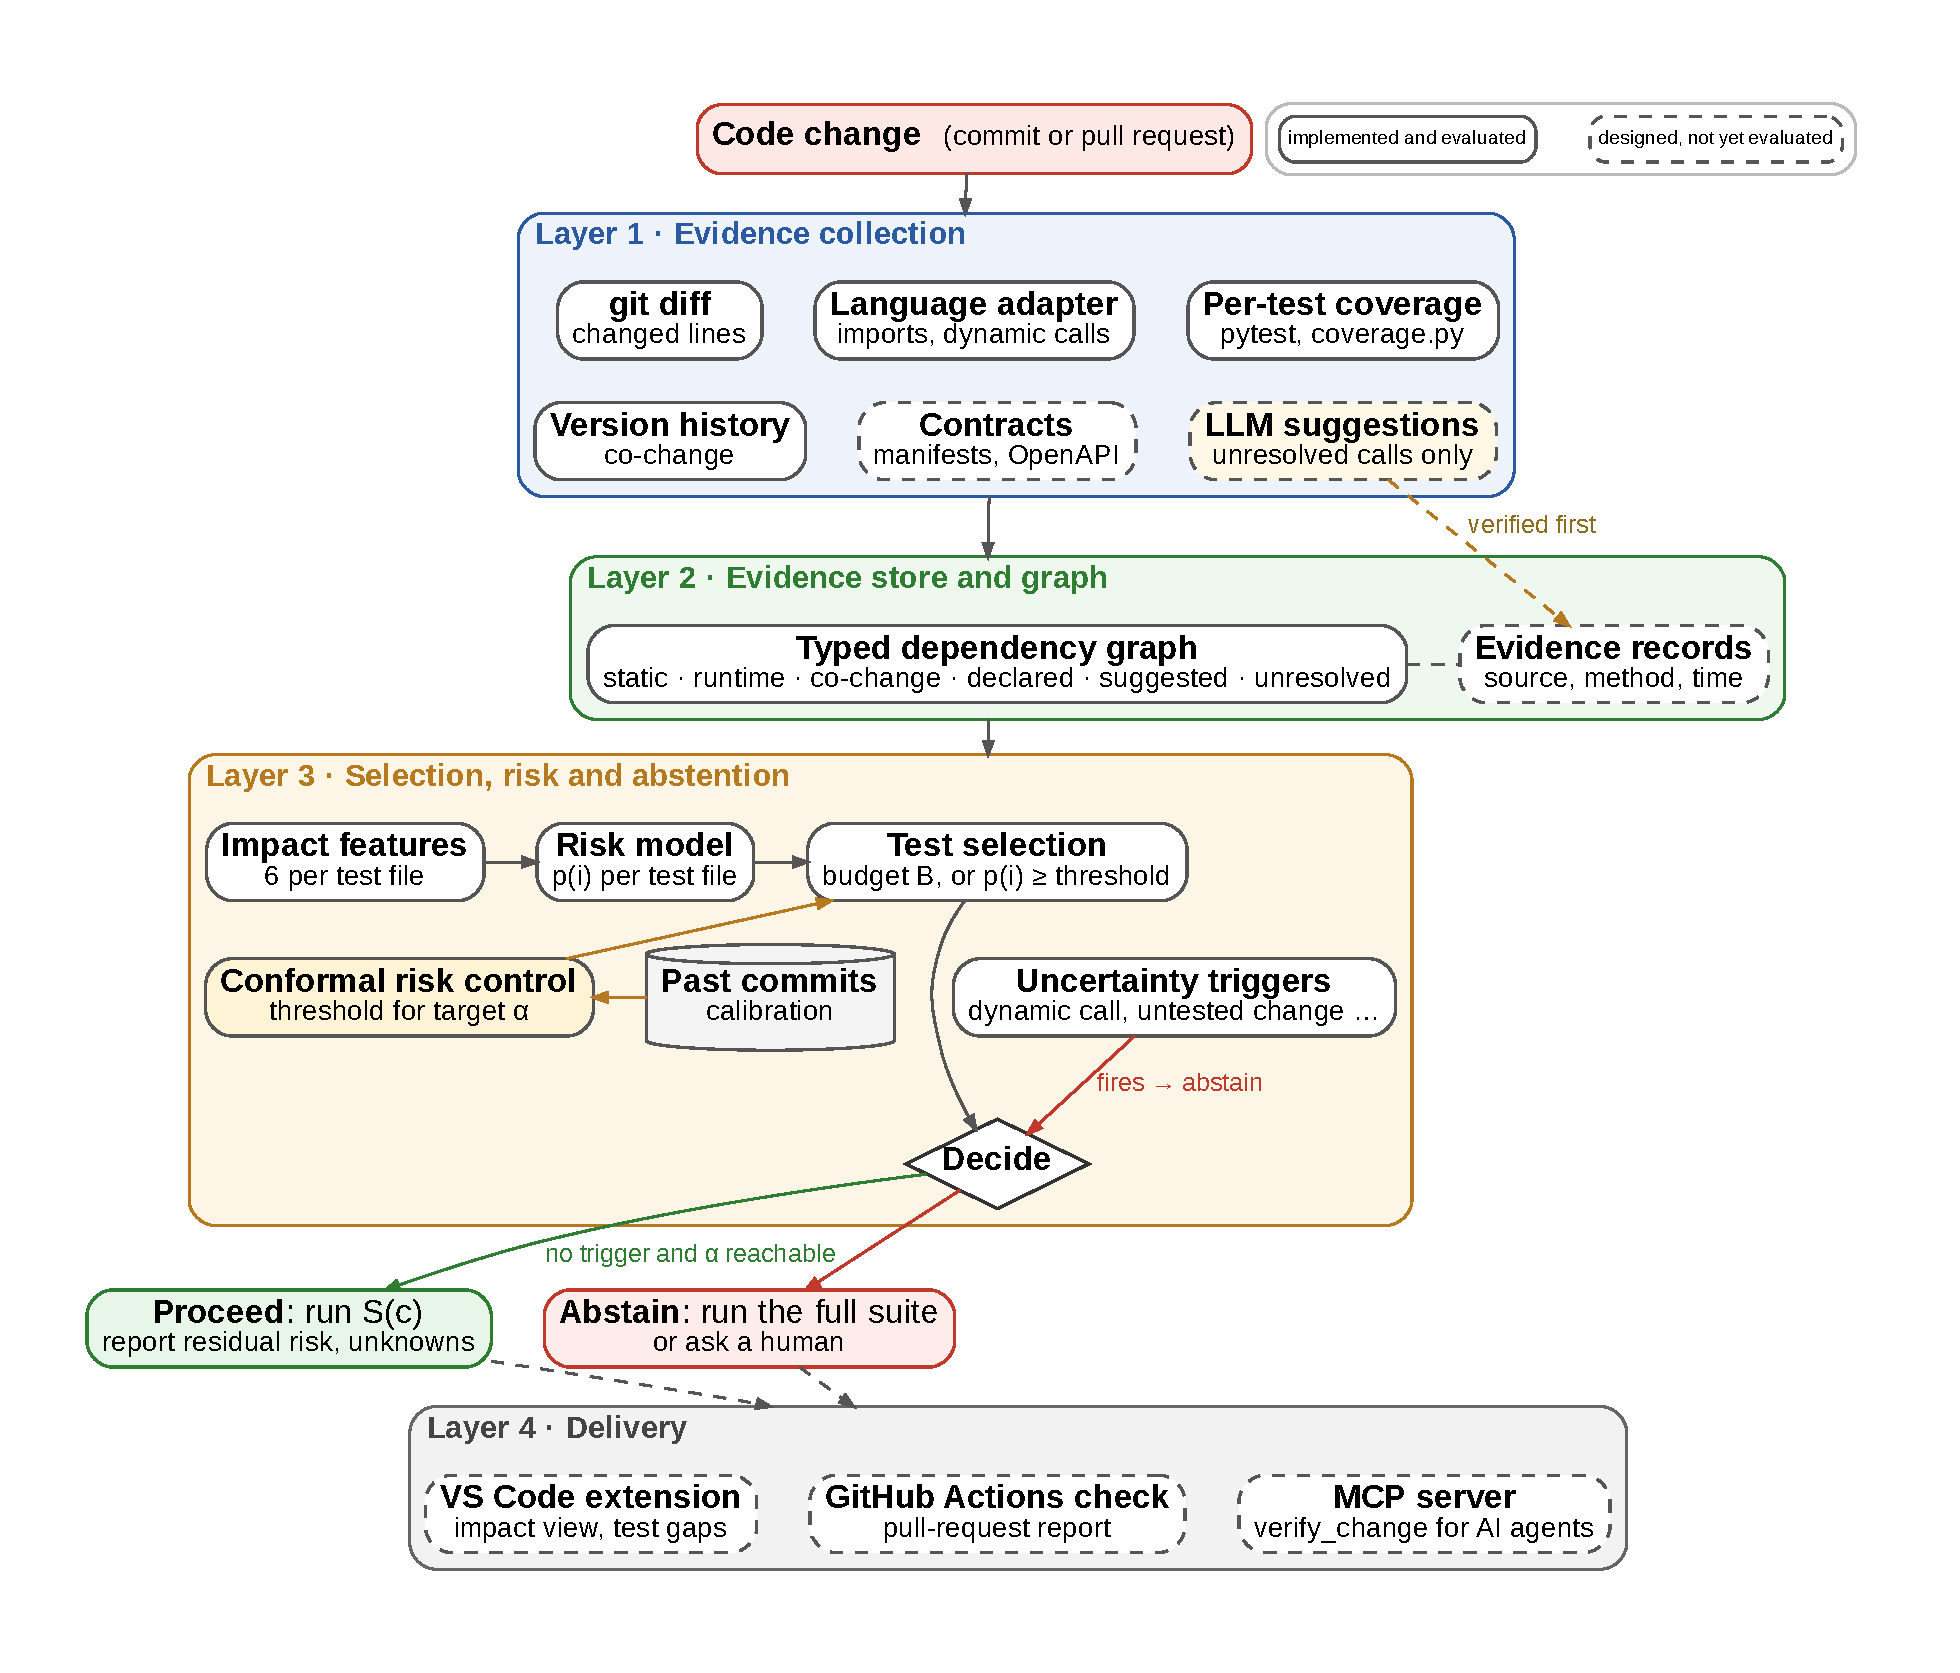
\includegraphics[width=0.85\textwidth]{figures/architecture_v2.pdf}}
\caption{Architecture and decision flow of CodeTwin AI. Layer~1 collects evidence about a change, Layer~2 stores it in a typed dependency graph, and Layer~3 scores each test file, selects tests within a budget or above a threshold calibrated on recent commits, and abstains to a broader run when the estimated residual risk exceeds the target (rule-based uncertainty triggers are evaluated as an alternative). Layer~4 delivers the decision. Solid boxes are implemented and evaluated in this paper; dashed boxes are designed but not yet evaluated.}
\label{fig:arch}
\end{figure*}

\subsection{Blind-Spot-Aware Evidence Graph}
Nodes of the graph represent files, functions, classes, tests, API endpoints and configuration keys. Every edge carries one evidence type: \emph{static} (found in the syntax tree), \emph{runtime-observed} (recorded by per-test coverage), \emph{declared} (taken from a manifest or API contract), \emph{co-change} (files that repeatedly change together in the version history), \emph{suggested} (proposed by a language model but not yet verified) or \emph{unresolved} (a link the analysis knows exists but cannot resolve, such as a \texttt{getattr} call with a computed name). Each record also stores its source location, the tool that produced it and a timestamp, so that stale evidence can be recognised. Unresolved edges are kept and counted, so that the report states what the analysis could not see instead of treating it as ``no dependency''. In the example of Fig.~\ref{fig:example}, the four dependants of the renamed field are connected by four different evidence types. Every link can be shown to the user as an \emph{evidence card}: the claim, its source file, line and commit, the method that produced it, the time and tool version, and its status (verified, inferred or unknown).

For every source file the prototype also records three line-level facts of each version: the span of every function (including its decorators), the lines that contain a dynamic call (\texttt{eval}, \texttt{exec}, \texttt{\_\_import\_\_}, \texttt{import\_module}, or \texttt{getattr}/\texttt{setattr}/\texttt{hasattr} with a computed name), and the lines of statements that run at import time (module-level and class-level statements other than imports, docstrings and plain constants, and all decorators). From this evidence it computes seven features for every pair of a change and a test file $i$, using only the previous version's coverage and the new version's static facts and diff: (1)~$x_{\mathit{line}}$, whether $i$ executed a changed line; (2)~$x_{\mathit{func}}$, whether $i$ executed the body of a function that encloses a changed line or insertion point; (3)~$x_{\mathit{file}}$, whether $i$ executed any changed file; (4)~$x_{\mathit{imp}}=1/d$, where $d$ is the import distance from $i$ to a changed module (depth at most six; $0$ if unreachable); (5)~$x_{\mathit{name}}$, whether the name of $i$ contains the name of a changed module; (6)~$x_{\mathit{co}}$, the share of the last 300 commits touching the changed files that also touched $i$; and (7)~$x_{\mathit{chg}}$, whether $i$ itself was added or changed.

The changed lines come from a zero-context \texttt{git diff} between the evaluated parent and the change. The coverage of the parent is matched against the \emph{old} line numbers, so no information from running the tests of the change is used. Lines that coverage.py records outside any test context are treated as import-time lines. The import graph is built from every \texttt{import} and \texttt{from}\ldots\texttt{import} statement; relative imports are resolved against the package path.

\subsection{Budgeted, Risk-Ranked Test Selection}\label{sec:select}
A logistic regression model with balanced class weights estimates the probability that test file $i$ is affected:
\begin{equation}
p(i) = \sigma\!\left(\mathbf{w}^{\top}\mathbf{x}_i + b\right), \label{eq:model}
\end{equation}
where $\mathbf{x}_i$ is the feature vector above and $\sigma$ the logistic function. In budget mode (Algorithm~\ref{alg:select}, lines 1--7) the tests in $F(c)$ are selected first; the remaining tests are then added in decreasing order of $p(i)/t(i)$, the most risk covered per second first, as long as the budget allows. This is the classical greedy rule for a knapsack problem in which a test's value is its probability of being affected and its weight is its run time. In calibrated mode (lines 8--14) every test with $p(i)\ge\hat\lambda_c$ is selected, where $\hat\lambda_c$ is a calibrated threshold (Section~\ref{sec:crc}), unless the system abstains. We chose logistic regression because the training data are small, because its weights can be inspected (Section~\ref{sec:ablation}), and because its scores grow monotonically with each feature.

\begin{algorithm}[t]
\caption{Risk-ranked selection with calibrated abstention}
\label{alg:select}
\begin{algorithmic}[1]
\Require tests $T$, forced tests $F$, scores $p(i)$, times $t(i)$, budget $B$, target $\alpha$, level $\alpha_c$, recent changes $\mathcal{C}$
\Ensure selected tests $S$, decision $d$
\Statex \textit{Budget mode}
\State $S \gets F$;\ $u \gets \sum_{i\in F} t(i)$
\For{$i \in T\setminus F$ in decreasing order of $p(i)/t(i)$}
  \If{$u + t(i) \le B$}
    \State $S \gets S \cup \{i\}$;\ $u \gets u + t(i)$
  \EndIf
\EndFor
\State \Return $S$
\Statex \textit{Calibrated mode}
\State $\hat\lambda_c \gets$ CRC threshold on $\mathcal{C}$ at level $\alpha_c$ \Comment{Eq.~(\ref{eq:crc})}
\State $S \gets F \cup \{\, i \in T : p(i) \ge \hat\lambda_c \,\}$
\If{$r(c) > \alpha$} \Comment{Eq.~(\ref{eq:rc})}
  \State \Return $S \cup S_{\mathit{broad}}$, \textsc{Abstain} \Comment{broader run}
\EndIf
\State \Return $S$, \textsc{Proceed}
\Statex \textit{After the change's tests run:} $\alpha_{c+1} \gets \alpha_c + \gamma(\alpha - \mathit{err}_c)$
\end{algorithmic}
\end{algorithm}

\subsection{Calibrated Selection Under Drift}\label{sec:crc}
The threshold is chosen with conformal risk control~\cite{angelopoulos2024crc}. The risk model is trained only on other projects. For a set $\mathcal{C}$ of $n$ earlier changes of the same project and a candidate threshold $\lambda$, the loss of change $c_j$ is one if some affected test outside $F(c_j)$ would be left out:
\begin{equation}
L_j(\lambda) = \mathbf{1}\big\{\exists\, i \in A(c_j)\setminus F(c_j) : p(i) < \lambda\big\}, \label{eq:loss}
\end{equation}
with empirical risk $\hat R_n(\lambda) = \tfrac{1}{n}\sum_{j=1}^{n} L_j(\lambda)$. Because the loss is bounded by one and does not decrease as $\lambda$ grows, the threshold
\begin{equation}
\hat\lambda = \sup\Big\{\lambda : \tfrac{n}{n+1}\hat R_n(\lambda) + \tfrac{1}{n+1} \le \alpha\Big\} \label{eq:crc}
\end{equation}
keeps the expected miss rate at or below $\alpha$ when the changes are exchangeable~\cite{angelopoulos2024crc}. The candidate thresholds are the smallest scores of affected tests on the calibration changes together with $0$ and $1$, so the supremum is found exactly. If no $\lambda$ qualifies, which happens whenever $\alpha < 1/(n+1)$, every test is selected.

Commits are ordered in time, and projects change: tests are reorganised, modules split, and the distribution of scores shifts. We therefore compare three ways of choosing $\mathcal{C}$ and the level. \emph{Static} calibration uses the first 40\% of a project's changes once, as in our earlier study. \emph{Sliding-window} calibration recomputes $\hat\lambda$ for every change from the $n$ most recent earlier changes, where $n$ is the size of the static calibration set. \emph{Adaptive} calibration additionally applies adaptive conformal inference (ACI)~\cite{gibbs2021aci}: after the tests of change $c$ have run, the level is updated as
\begin{equation}
\alpha_{c+1} = \alpha_c + \gamma\,(\alpha - \mathit{err}_c), \label{eq:aci}
\end{equation}
where $\mathit{err}_c\in\{0,1\}$ records whether the selection missed an affected test and $\gamma=<<ACI_GAMMA>>$. A miss lowers the level used for later changes, which raises their selection; a run of safe changes slowly relaxes it. ACI guarantees that the long-run miss rate approaches $\alpha$ without any assumption on how the data shift~\cite{gibbs2021aci}. Both time-aware variants need the true outcome of earlier changes; in practice it comes from post-merge or nightly full runs, which teams that use selection usually keep~\cite{machalica2019pts,memon2017taming}.

\subsection{Residual Risk and Abstention}\label{sec:risk}
For one change, CodeTwin AI estimates the probability that its selection misses an affected test. The model scores of the calibration changes are first recalibrated with isotonic regression~\cite{zadrozny2002calibration}, which maps a score to the observed frequency of affected tests, giving $\tilde p(i)$. Treating skipped tests as independent,
\begin{equation}
r(c) = 1 - \textstyle\prod_{i \in T\setminus S(c)} \big(1-\tilde p(i)\big). \label{eq:rc}
\end{equation}
The system abstains when $r(c)$ exceeds the target $\alpha$. As the broader run we compare three options: the full suite, file-coverage selection (every test that executed a changed file) and the hybrid of static reachability and file coverage, each joined with the calibrated selection. We also evaluate the rule-based uncertainty triggers of the design (Table~\ref{tab:triggers}). The prototype implements the four triggers that need only single-repository evidence in two forms: \emph{file-level}, as in our earlier study, where a trigger fires when any changed file contains a dynamic call, any changed line ran at import time, and so on; and \emph{line-level}, where only the changed lines and the functions that enclose them count. The line-level module trigger uses the static import-time statements of the new version instead of the new test run.

\begin{table}[t]
\caption{Uncertainty Triggers}
\label{tab:triggers}
\centering
\footnotesize
\setlength{\tabcolsep}{3pt}
\begin{tabular}{@{}>{\raggedright\arraybackslash}p{0.24\columnwidth}>{\raggedright\arraybackslash}p{0.56\columnwidth}>{\raggedright\arraybackslash}p{0.13\columnwidth}@{}}
\toprule
\textbf{Trigger} & \textbf{Fires when (line-level form)} & \textbf{Status} \\
\midrule
Dynamic call & a changed line, or the function enclosing it, contains a dynamic call & evaluated \\
Untested change & no test executed the function enclosing a changed line, an edited import-time statement, or a new module & evaluated \\
Static/runtime conflict & a test executed a changed line but has no static import path to it & evaluated \\
Module-level change & a changed line is an import-time statement, so every importer is affected & evaluated \\
\midrule
Risk & $r(c) > \alpha$ (Eq.~\ref{eq:rc}) & evaluated \\
\midrule
Unknown consumer & a cross-repository link cannot be resolved & planned \\
Stale evidence & coverage or dependency data are older than the code & planned \\
Hidden coupling & files often change together with no code link & planned \\
Unparsed file & a changed file has no adapter or cannot be parsed & planned \\
\bottomrule
\end{tabular}
\end{table}

\subsection{Role of Machine Learning and Language Models}
Where static analysis stops, for example at a \texttt{getattr} call with a computed name, we design a locally run language model to read the surrounding code and propose likely targets. Because language models alone build less complete call graphs than static tools~\cite{venkatesh2025llmcg}, a suggestion enters the graph only with the type \emph{suggested}. It is promoted to \emph{verified} after a small probe test confirms that the call reaches the proposed target, and it never lowers the risk estimate before that.

The framework follows one principle: \emph{analysis computes, the model suggests}. Facts about the code come from program analysis and test runs; machine learning turns them into a risk estimate (Section~\ref{sec:select}), and statistics checks whether that estimate is honest (Section~\ref{sec:risk}). Besides link suggestion, three further model-based components are designed, each subordinate to evidence. \emph{Retrieval} searches non-code files such as configuration, templates and documentation, other repositories and past CI logs for dynamic uses of a changed name, and returns each hit with its source. \emph{Targeted test generation} asks a language model to write a test only for a path that no test executes; the test is run before it is accepted, and the drop in residual risk is shown. \emph{Explanation} turns evidence records into readable text and may not add any fact that is not in a record. Four rules control the risk of these components: a suggested link stays ``suggested'' until a probe or test confirms it; generated text may only restate evidence records; the effect of suggestions on the miss rate is measured and reported even if it is negative; and seeds, model and tool versions and the list of evaluated commits are recorded for repeatability. None of these model-based components was implemented or evaluated in this study.

\subsection{Developer and Agent Interfaces}
The design delivers the same analysis through three interfaces, summarised in Table~\ref{tab:interfaces}. The \emph{VS Code extension} is the main interface, because the developer selects code there and can see its impact before making a change. A \emph{GitHub Actions check} runs the same analysis on every pull request and posts a comment with the affected components, the selected tests, the residual risk, the unknowns and the recommendation; as a \emph{risk-bearing receipt}, it can allow a merge only when the residual risk is below the team's target or a named reviewer has accepted the risk. An \emph{MCP server} exposes the engine to AI coding agents, so that an agent can ask, before it opens a pull request, whether its change is safe to submit. The agent receives the same calibrated answer as a developer and cannot override it: if CodeTwin AI abstains, the agent is told to run more tests or to ask a human. Existing agent support gives a fixed code-to-test map~\cite{alonso2026tdad}; the MCP server adds a calibrated stop-or-go decision while reusing the same engine. These interfaces were not part of the evaluated prototype, and GitHub Actions was used only to run the experiments (Section~\ref{sec:impl}). A first version of the select-to-impact panel, the MCP tools of Table~\ref{tab:interfaces} and a GitHub Actions step that reports the selection and its risk have since been implemented in the CodeTwin AI tool (release 0.1.0); they are not evaluated in this paper, and the pull-request comment and the risk-bearing receipt are not implemented yet.

\begin{table}[t]
\caption{Planned Developer and Agent Interfaces}
\label{tab:interfaces}
\centering
\footnotesize
\setlength{\tabcolsep}{3pt}
\begin{tabular}{@{}>{\raggedright\arraybackslash}p{0.33\columnwidth}>{\raggedright\arraybackslash}p{0.62\columnwidth}@{}}
\toprule
\textbf{Feature} & \textbf{What the user receives} \\
\midrule
\multicolumn{2}{@{}l}{\textit{VS Code extension}} \\
Select-to-impact & a side panel with callers, callees, tests and consumers of the selected code; line style shows the evidence type, dotted lines show unresolved links \\
Impact CodeLens & a line above each function, e.g.\ ``used by 7 $\cdot$ 2 repos $\cdot$ 5 tests $\cdot$ 1 unknown'' \\
Blind-spot highlighting & shading of \texttt{getattr}, \texttt{importlib} and \texttt{eval} lines that the analysis cannot follow \\
Test-gap gutter & a mark on changed lines that no test executes \\
Recommended tests & ranked tests, budget and residual risk, runnable from the Test Explorer \\
\midrule
\multicolumn{2}{@{}l}{\textit{GitHub Actions pull-request check}} \\
Pull-request report & affected components, selected tests, residual risk, unknowns and recommendation \\
Risk-bearing receipt & merge allowed only below the target risk or with a reviewer's sign-off \\
\midrule
\multicolumn{2}{@{}l}{\textit{MCP server for AI coding agents}} \\
\texttt{verify\_change} & affected components, tests, residual risk, unknowns and a decision: proceed, run\_more or ask\_human \\
\texttt{get\_impact} & the impact map of a symbol or file with the evidence type of every link \\
\texttt{recommend\_tests} & ranked tests within a given budget, each with its reason \\
\texttt{explain\_decision} & the evidence records behind a recommendation \\
\bottomrule
\end{tabular}
\end{table}

\subsection{Planned Extensions}
The same rule, in which a model or heuristic proposes, evidence verifies, risk is calibrated and the tool abstains when unsure, extends to further features that are planned after the core is evaluated. \emph{Active link verification} runs a small probe for the uncertain links whose confirmation would lower the residual risk most. An \emph{evidence freshness meter} raises the risk as coverage and dependency data age. A \emph{consumer-evidence contract check} links every API or schema change to consumer code and tests in other repositories, and a \emph{cross-repository collision radar} warns when open pull requests in different repositories have overlapping impact. A \emph{flaky-evidence discount} treats a pass from a flaky test as weaker evidence. A \emph{conformal culprit set} reports, for a failing test, the small set of commits that contains the cause with a chosen confidence, and a \emph{promise monitor} tracks the observed miss rate against the promised target over time and alerts on drift.

% =====================================================================
\section{Implementation}\label{sec:impl}
% =====================================================================
The prototype consists of three Python scripts. The \emph{collector} (<<LOC_COLLECT>> lines) checks out each evaluated change and its parent, records the diff, the static facts of every file with the Python \texttt{ast} module, and runs the test suite with pytest~8, pytest-cov and coverage.py (C tracer, one coverage context per test) to obtain per-test-file coverage, run times and per-test-case outcomes. It then seeds up to three faults on changed lines of the new version (Section~\ref{sec:gt}) and runs the test files that executed the mutated file, with a per-test timeout so that a hanging test counts as failing. The \emph{analysis} script (<<LOC_ANALYZE>> lines) computes the ground truths, baselines, risk model (scikit-learn logistic regression and isotonic regression), the three calibration variants, residual risk, triggers, abstention, ablation, bootstrap confidence intervals and paired tests with SciPy. A third script writes every number of this paper from the analysis output, so no result is typed by hand.

The experiments ran on GitHub Actions with Python~3.12. One workflow splits the changes of each project into contiguous shards and runs <<N_SHARDS>> collection jobs in parallel on Ubuntu runners; a final job merges the data and runs the analysis. The commit list is fixed by a cutoff date (10 November 2026), so a rerun selects the same changes. For the NameRTS projects we installed each project's test dependencies once from its newest commit and pinned the pandas and NumPy versions of the NameRTS replication environment, so that older commits still run. After the study, the evidence store (SQLite), a first VS Code extension, a GitHub Actions step and the MCP server were implemented in the CodeTwin AI tool (release 0.1.0) on the same scoring, calibration and abstention code; they were not used in these experiments. The language-model link suggestions, the pull-request comment and receipt, cross-repository evidence and adapters for other languages are not implemented yet.

% =====================================================================
\section{Experimental Setup}\label{sec:setup}
% =====================================================================
\subsection{Research Questions}
We answer the research question of the Introduction through four research questions, which test the hypotheses H1 to H3 of the project synopsis; H4 (verified language-model suggestions) is left for future work.

\textbf{RQ1 (selection quality, H1).} At the same time budget, does risk-ranked selection find more affected tests than simpler baselines? A method that saves time is only useful if it still finds the tests a change can break.

\textbf{RQ2 (calibration, H2).} Does the observed miss rate on later changes stay at or below the target $\alpha$, and does the per-change estimate $r(c)$ match how often selections actually miss? This checks whether the stated risk can be trusted on changes the system has not seen.

\textbf{RQ3 (abstention, H3).} Do uncertainty triggers and risk-based abstention flag the changes on which conventional selection misses tests, at an acceptable abstention rate and cost?

\textbf{RQ4 (faults and NameRTS).} Do the selections detect seeded faults, and how does CodeTwin AI compare with NameRTS on NameRTS's own changes and ground truth?

\subsection{Subject Projects}
Table~\ref{tab:subjects} lists the subjects. The five \emph{history} projects (click, python-dateutil, itsdangerous, marshmallow and toolz) are open-source Python libraries with pytest suites. For each we took up to the last 250 mainline commits before the cutoff that change at least one source file, and compared each with the previous one; merge commits are included because most changes enter these projects as pull-request merges. Changes whose old or new version could not be tested with per-test coverage on Python~3.12 were dropped (<<NO_COV>> changes, mostly old commits of toolz and marshmallow), and dateutil has only <<DATEUTIL_CHANGES>> source-changing mainline commits since it moved to its current source layout. The <<N_NRTS_PROJ>> \emph{NameRTS} projects use exactly the commit pairs of the NameRTS replication package~\cite{wang2026namerts}: for each of its target commits we compare the commit with the parent that NameRTS used. In total we evaluated <<N_CHANGES>> changes, with <<N_HIST_TEST>> test changes on the history projects and <<N_NRTS_TEST>> on the NameRTS projects.

\begin{table}[t]
\caption{Subject Projects}
\label{tab:subjects}
\centering
\footnotesize
\setlength{\tabcolsep}{1.8pt}
\begin{tabular}{@{}lrrrrrrr@{}}
\toprule
\textbf{Project} & \textbf{Changes} & \textbf{KLoC} & \textbf{Tests} & \textbf{Suite} & \textbf{Aff.} & \textbf{Mut.} & \textbf{Years} \\
\midrule
<<TAB_SUBJECTS>>
\bottomrule
\multicolumn{8}{@{}p{0.97\columnwidth}@{}}{Changes = evaluated changes (calibration/test); Tests = mean test files; Suite = mean full-suite time with coverage (s); Aff.\ = mean affected test files per change; Mut.\ = seeded faults detected by at least one test. $^\ast$NameRTS commit pairs.}
\end{tabular}
\end{table}

\subsection{Ground Truths}\label{sec:gt}
\emph{Coverage.} A test file is \textit{affected} by a change if, in the new version, (a)~it executes a changed source line (per-test coverage contexts); (b)~it executes a module whose import-time code changed; (c)~the test file itself was added or changed; or (d)~it executed, in the old version, a source file that the change deleted. Coverage shows which tests could notice a change, not which would fail.

\emph{Seeded faults.} To measure fault detection, we seeded up to three mutants per change on changed lines of the new version, chosen at random on different lines, with nine classic operators~\cite{jia2011mutation}: relational, arithmetic and logical operator replacement, negation removal, Boolean and integer constant replacement, return-value replacement, call-statement deletion and assignment-value replacement. A test file \emph{detects} a mutant if one of its test cases that passed on the unmutated code fails. Each mutant is run against the test files that executed the mutated file. Mutants that no test detects (survivors, including equivalent mutants) and mutants whose run timed out or failed to start are excluded. Mutant detection correlates with real-fault detection~\cite{just2014mutants}.

\emph{NameRTS.} On the NameRTS projects we also use the published NameRTS ground truth of affected test files~\cite{wang2026namerts}, restricted to the test files that exist in our runs.

\subsection{Baselines}
\textit{Retest-all} runs every test file. \textit{Name matching} selects test files whose name contains the name of a changed module, a simple heuristic inspired by NameRTS~\cite{wang2026namerts}. \textit{Static import} selects test files that reach a changed module through the import graph, as static class- or file-level RTS does~\cite{legunsen2016static}. \textit{File coverage} selects tests that executed a changed file in the previous version, in the style of Ekstazi~\cite{gligoric2015ekstazi}; \textit{Function coverage} and \textit{Line coverage} require that they executed a changed function or line. \textit{Hybrid} is the union of static import and file coverage. Every baseline also runs added or changed test files. Under a time budget, \textit{Random} ranks test files randomly (20 seeds) and \textit{Coverage-ranked} by a fixed weighted sum of the coverage and import features. On the NameRTS projects we also evaluate the \textit{published NameRTS selections}, so NameRTS itself, not a re-implementation, is compared.

\subsection{Metrics}
With $T$, $t(i)$, $A(c)$ and $S(c)$ as before, we report test reduction $1-|S|/|T|$, time reduction $1-\sum_{i\in S}t(i)/\sum_{i\in T}t(i)$, precision $|S\cap A|/|S|$ and recall $|S\cap A|/|A|$, each averaged over changes (precision and recall over changes with at least one affected test). A selection is \textit{safe} for a change if $A(c)\subseteq S(c)$; the observed miss rate is the share of unsafe changes. For seeded faults we report the \textit{mutant detection rate}, the share of detected mutants for which the selection contains at least one detecting test. For $r(c)$ we report the Brier score~\cite{brier1950verification}, the mean squared difference between $r(c)$ and the observed miss (0 or 1), compared with a constant forecast, and the expected calibration error over five bins. Run times are the measured times of the new version.

\subsection{Protocol}
Fig.~\ref{fig:workflow} summarises the study. Each project's changes are ordered in time. The first 40\% calibrate and the rest are test changes; calibration changes are never used for training. The risk model is trained leave-one-project-out on the other history projects; the NameRTS projects use a model trained on all history projects. Budgets are 10\%, 25\% and 50\% of the previous version's full-suite time, and targets are $\alpha\in\{0.01,0.05,0.10,0.20\}$; the sliding window and ACI start from the same calibration set, and ACI uses $\gamma=<<ACI_GAMMA>>$, fixed in advance. Isotonic recalibration for $r(c)$ is fitted on the calibration changes. For the ablation we retrain the model without one evidence signal, or without all coverage signals, and compare at the 25\% budget. We report 95\% bootstrap confidence intervals (10,000 resamples over test changes) and paired Wilcoxon signed-rank tests for recall.

% =====================================================================

\begin{figure*}[t]
\centering
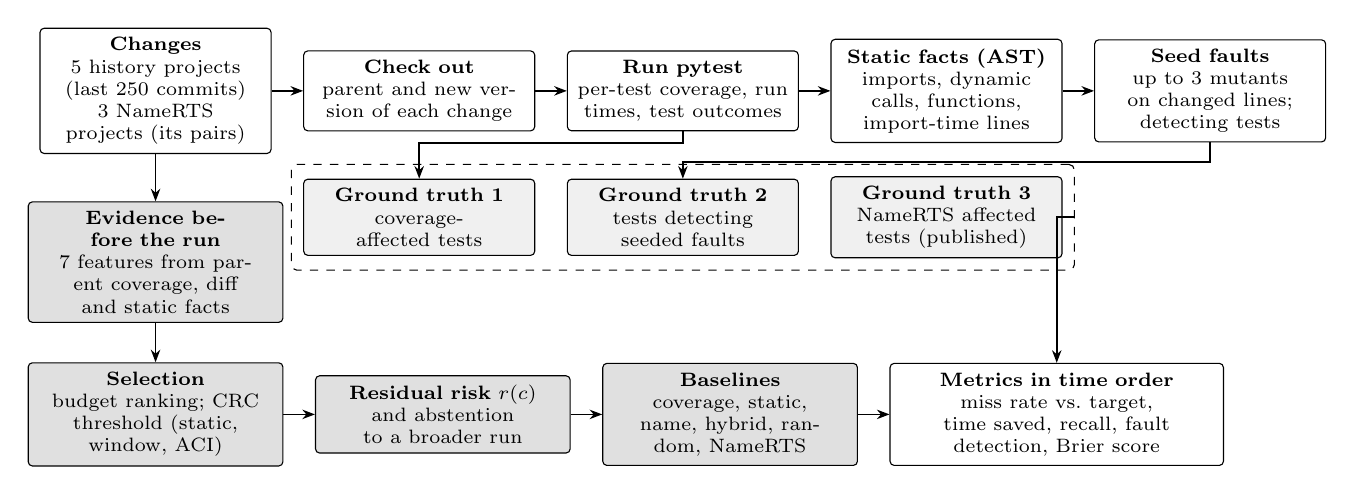
\begin{tikzpicture}[font=\scriptsize, node distance=3.5mm and 4mm,
  box/.style={draw, rounded corners=1.5pt, align=center, minimum height=9mm, text width=27mm, fill=white},
  gt/.style={box, fill=black!6}, an/.style={box, text width=30mm, fill=black!12},
  arr/.style={-{Stealth[length=1.6mm]}, semithick}]
\node[box] (hist) {\textbf{Changes}\\ 5 history projects (last 250 commits)\\ 3 NameRTS projects (its pairs)};
\node[box, right=of hist] (co) {\textbf{Check out}\\ parent and new version of each change};
\node[box, right=of co] (run) {\textbf{Run pytest}\\ per-test coverage, run times, test outcomes};
\node[box, right=of run] (st) {\textbf{Static facts (AST)}\\ imports, dynamic calls, functions, import-time lines};
\node[box, right=of st] (mut) {\textbf{Seed faults}\\ up to 3 mutants on changed lines; detecting tests};
\node[gt, below=6mm of co] (g1) {\textbf{Ground truth 1}\\ coverage-affected tests};
\node[gt, right=of g1] (g2) {\textbf{Ground truth 2}\\ tests detecting seeded faults};
\node[gt, right=of g2] (g3) {\textbf{Ground truth 3}\\ NameRTS affected tests (published)};
\node[an, below=6mm of hist] (f) {\textbf{Evidence before the run}\\ 7 features from parent coverage, diff and static facts};
\node[an, below=5mm of f] (sel) {\textbf{Selection}\\ budget ranking; CRC threshold (static, window, ACI)};
\node[an, right=of sel] (risk) {\textbf{Residual risk} $r(c)$\\ and abstention to a broader run};
\node[an, right=of risk] (base) {\textbf{Baselines}\\ coverage, static, name, hybrid, random, NameRTS};
\node[box, right=of base, text width=40mm] (met) {\textbf{Metrics in time order}\\ miss rate vs.\ target, time saved, recall, fault detection, Brier score};
\draw[arr] (hist) -- (co); \draw[arr] (co) -- (run); \draw[arr] (run) -- (st); \draw[arr] (st) -- (mut);
\draw[arr] (run.south) -- ++(0,-1.5mm) -| (g1.north);
\draw[arr] (mut.south) |- ++(0,-2.5mm) -| (g2.north);
\draw[arr] (hist.south) -- (f.north);
\draw[arr] (f) -- (sel); \draw[arr] (sel) -- (risk); \draw[arr] (risk) -- (base); \draw[arr] (base) -- (met);
\node[draw, dashed, rounded corners=2pt, inner sep=1.5mm, fit=(g1)(g2)(g3)] (gts) {};
\draw[arr] (gts.east) -| (met.north);
\end{tikzpicture}
\caption{Study workflow. Collection (top row) runs on GitHub Actions in 52 parallel shards; the analysis (bottom row) processes each project's changes in time order and uses the new version's test run only for the ground truths.}
\label{fig:workflow}
\end{figure*}
\section{Results}\label{sec:results}
% =====================================================================
\subsection{RQ1: Selection Quality}
Table~\ref{tab:rq1} compares all techniques over the <<N_HIST_TEST>> test changes of the history projects. The baselines span a clear trade-off. File coverage and the hybrid never missed an affected test but saved only <<FILE_TIME>>\% and <<HYB_TIME>>\% of test time. Function and line coverage saved <<FUNC_TIME>>\% and <<LINE_TIME>>\% but were unsafe on <<FUNC_MISS>>\% and <<LINE_MISS>>\% of changes. Name matching saved the most time (<<NAME_TIME>>\%) but had a recall of only <<NAME_RECALL>>. Function coverage, which we expected to fix the misses of line coverage, was less safe: when a change edits a function's signature or decorator, which run at import time, line coverage keeps every test that loaded the module, whereas function coverage keeps only the tests that ran the function body.

\begin{table}[t]
\caption{Selection Quality on the History Projects (Mean Over <<N_HIST_TEST>> Test Changes)}
\label{tab:rq1}
\centering
\footnotesize
\setlength{\tabcolsep}{1.6pt}
\begin{tabular}{@{}lrrrrrr@{}}
\toprule
\textbf{Technique} & \textbf{TestR\%} & \textbf{TimeR\%} & \textbf{Prec.} & \textbf{Rec.} & \textbf{Safe\%} & \textbf{Mut.\%} \\
\midrule
<<TAB_RQ1>>
\bottomrule
\multicolumn{7}{@{}p{0.97\columnwidth}@{}}{Mut.\% = share of detected seeded faults for which the selection contains a detecting test.}
\end{tabular}
\end{table}

Fig.~\ref{fig:budget} shows budget mode. At 10, 25 and 50\% of full-suite time, the learned ranking reached a recall of <<B10_CT_RECALL>>, <<B25_CT_RECALL>> and <<B50_CT_RECALL>>. It beat random selection at every budget (paired Wilcoxon tests, $p<<P_B10_RND>>$, $p<<P_B25_RND>>$ and $p<<P_B50_RND>>$; mean differences <<D_B10_RND>>, <<D_B25_RND>> and <<D_B50_RND>>) but was practically identical to the coverage ranking (<<B10_CR_RECALL>>, <<B25_CR_RECALL>> and <<B50_CR_RECALL>>; $p<<P_B10_CR>>$, $p<<P_B25_CR>>$ and $p<<P_B50_CR>>$). With a fixed budget at most <<B50_CT_SAFE>>\% of changes were safe, which is why a calibrated mode is needed.

Fig.~\ref{fig:tradeoff} places every technique by time saved and miss rate. The coverage baselines form the frontier on these projects; adaptive calibration moves along it as the target changes, and risk-based abstention sits just above file coverage, with slightly more time saved and a small miss rate.

\begin{figure}[t]
\centering
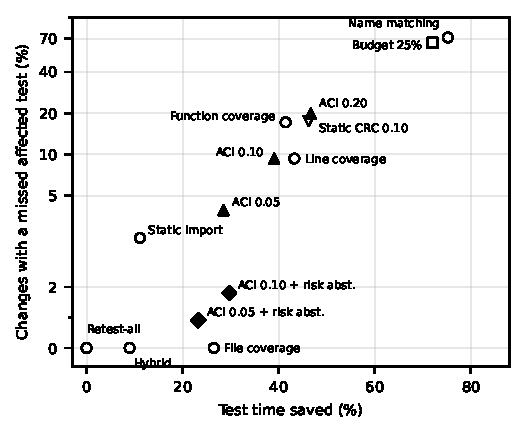
\includegraphics[width=\columnwidth]{figures/tradeoff.pdf}
\caption{Time saved against the share of changes with a missed affected test (history projects; vertical axis linear up to 5\%, then logarithmic). Circles: baselines; triangles: CodeTwin AI with adaptive calibration; diamonds: with risk-based abstention.}
\label{fig:tradeoff}
\end{figure}

\textbf{Answer to RQ1:} risk-ranked selection finds more affected tests than random selection within the same budget, but on these projects it adds nothing over a coverage ranking (H1 not supported against coverage-only selection).

\begin{figure}[t]
\centering
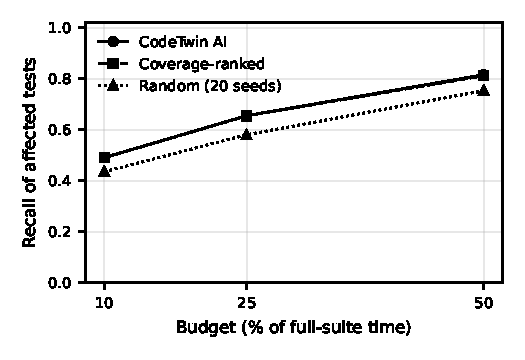
\includegraphics[width=\columnwidth]{figures/budget.pdf}
\caption{Recall of affected tests at different time budgets (history projects).}
\label{fig:budget}
\end{figure}

\subsection{RQ2: Calibration and Residual Risk}
Table~\ref{tab:rq2} and Fig.~\ref{fig:calib} report the observed miss rate for each target. Static calibration, fitted once on each project's oldest 40\% of changes, did not hold: for targets of 5\%, 10\% and 20\% it missed affected tests on <<CRC5_MISS>>\%, <<CRC10_MISS>>\% and <<CRC20_MISS>>\% of later changes. The worst case was <<WORST_STATIC_PROJ>>, where the threshold fitted on old changes (<<WORST_STATIC_LAMBDA>>) was too high for newer ones and <<WORST_STATIC_MISS>>\% of test changes were missed. The sliding window, which recalibrates on recent changes, came closer (<<WIN5_MISS>>\%, <<WIN10_MISS>>\% and <<WIN20_MISS>>\%). Adaptive calibration kept the miss rate at or below every target on the history projects: <<ACI1_MISS>>\%, <<ACI5_MISS>>\%, <<ACI10_MISS>>\% and <<ACI20_MISS>>\% for targets of 1\%, 5\%, 10\% and 20\%, while saving <<ACI5_TIME>>\%, <<ACI10_TIME>>\% and <<ACI20_TIME>>\% of test time at the three larger targets. At $\alpha=0.10$ its safety equalled that of line coverage (<<LINE_SAFE>>\%) with slightly less time saved, but the level is chosen in advance and can be tightened: at $\alpha=0.05$ it was safe on <<ACI5_SAFE_PCT>>\% of changes. Fig.~\ref{fig:perproject} shows that the pooled result hides variation: per history project, adaptive calibration missed between <<ACI10_PROJ_MIN>>\% and <<ACI10_PROJ_MAX>>\% of changes at $\alpha=0.10$ (highest for <<ACI10_PROJ_MAXNAME>>), so a single project can exceed the target by about a point; on the NameRTS commits the highest was <<NACI10_PROJ_MAX>>\% (<<NACI10_PROJ_MAXNAME>>). In our earlier study, with 15--16 calibration changes per project, static calibration appeared valid; with <<CALIB_MIN>>--<<CALIB_MAX>> calibration changes over longer periods, drift dominates.

\begin{table}[t]
\caption{Observed Miss Rate (\%) and Time Saved (\%) per Target $\alpha$ (History Projects)}
\label{tab:rq2}
\centering
\footnotesize
\setlength{\tabcolsep}{3pt}
\begin{tabular}{@{}lrrrrrr@{}}
\toprule
& \multicolumn{2}{c}{\textbf{Static}} & \multicolumn{2}{c}{\textbf{Sliding window}} & \multicolumn{2}{c}{\textbf{Adaptive (ACI)}} \\
\cmidrule(lr){2-3}\cmidrule(lr){4-5}\cmidrule(l){6-7}
$\alpha$ & Miss & Time & Miss & Time & Miss & Time \\
\midrule
<<TAB_RQ2>>
\bottomrule
\end{tabular}
\end{table}

\begin{figure}[t]
\centering
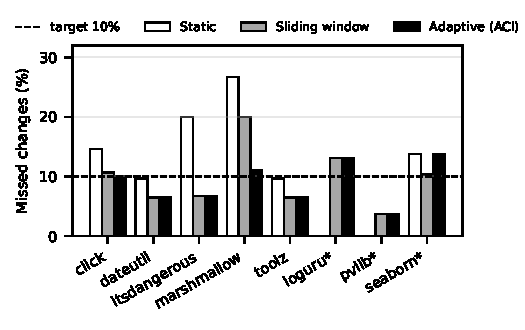
\includegraphics[width=\columnwidth]{figures/per_project.pdf}
\caption{Share of changes with a missed affected test per project at target $\alpha=0.10$ ($^\ast$NameRTS commits). A bar of zero means no miss.}
\label{fig:perproject}
\end{figure}

\begin{figure}[t]
\centering
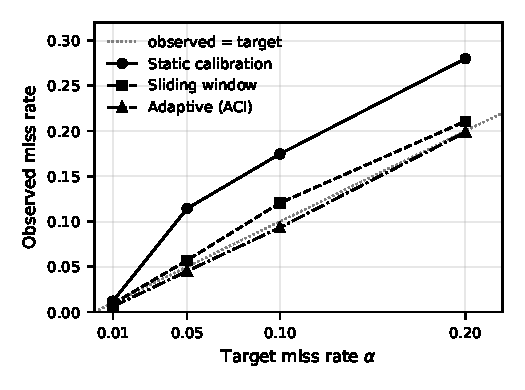
\includegraphics[width=\columnwidth]{figures/calibration.pdf}
\caption{Observed miss rate against the target $\alpha$ for the three calibration variants (history projects). Points below the dotted line meet the target.}
\label{fig:calib}
\end{figure}

The per-change estimate $r(c)$ separated risky from safe selections. In budget mode at 25\%, where selections are often unsafe, its mean was <<RB_PRED>>\% against an observed miss rate of <<RB_OBS>>\%, with a Brier score of <<RB_BRIER>> against <<RB_BRIER0>> for a constant forecast. For the adaptively calibrated selections at $\alpha=0.10$ it overestimated the risk (mean <<RC_PRED>>\% against <<RC_OBS>>\% observed; Brier <<RC_BRIER>> against <<RC_BRIER0>> for a constant forecast), probably because skipped tests are not independent, as Eq.~(\ref{eq:rc}) assumes: when one is affected, others often are too. It still separated changes well: the <<RC_LOW_N>> of <<RC_N>> changes with $r(c)<0.2$ were missed <<RC_LOW_OBS>>\% of the time, the <<RC_HI_N>> changes with $r(c)>0.8$ <<RC_HI_OBS>>\% of the time. Fig.~\ref{fig:reliability} shows the reliability diagram. Its value is therefore mainly in ranking changes by risk, which RQ3 uses.

\begin{figure}[t]
\centering
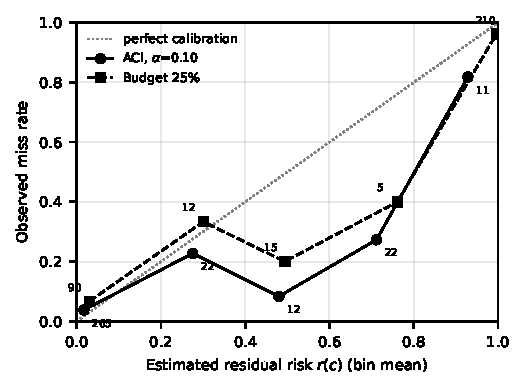
\includegraphics[width=\columnwidth]{figures/reliability.pdf}
\caption{Reliability of the residual-risk estimate $r(c)$ (history projects): mean estimate against observed miss rate in five bins; numbers give the changes per bin. Points below the diagonal overestimate the risk.}
\label{fig:reliability}
\end{figure}

\textbf{Answer to RQ2:} on the history projects the miss rate stays at the target only with calibration that adapts over time (H2 supported for ACI, not for static calibration); $r(c)$ ranks changes by risk but overestimates its level for calibrated selections.

\subsection{RQ3: Uncertainty Triggers and Risk-Based Abstention}
Line coverage was unsafe on <<TF_UNSAFE>> of the <<TF_TEST>> test changes (<<BASE_UNSAFE_RATE>>\%). The file-level triggers of our earlier study flagged <<TF_FLAG_UNSAFE>> of them but also fired on <<TF_FALSE>>\% of the safe changes. Restricting the triggers to changed lines halved the abstention rate but kept only <<TL_FLAG_UNSAFE>> of the <<TL_UNSAFE>> unsafe changes, a smaller share than of the safe ones (<<TL_FALSE>>\%): the line-level rules did not point at the changes that were actually risky. The risk rule $r(c)>\alpha$, applied to the line-coverage selection, flagged <<TR_FLAG_UNSAFE>> of the <<TR_UNSAFE>> unsafe changes while firing on only <<TR_FALSE>>\% of the safe ones.

Fig.~\ref{fig:triggers} contrasts the three rules.

\begin{figure}[t]
\centering
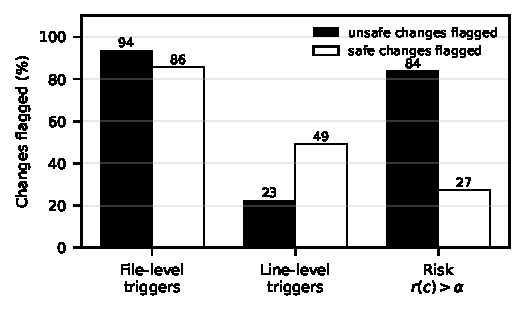
\includegraphics[width=\columnwidth]{figures/triggers.pdf}
\caption{Share of unsafe and of safe changes (for line-coverage selection) that each abstention rule flags (history projects). A useful rule flags many unsafe and few safe changes.}
\label{fig:triggers}
\end{figure}

Table~\ref{tab:rq3} shows the cost of each policy on top of adaptive calibration at $\alpha=0.10$. File-level triggers made almost every change safe but abstained on <<AF_RATE>>\% of changes, leaving <<AF_FULL_TIME>>\% saving with a full-suite fallback. Risk-based abstention fired on <<AR_RATE>>\% of changes; with file-coverage selection as the broader run, <<AR_FILECOV_SAFE>>\% of changes were safe and <<AR_FILECOV_TIME>>\% of test time was saved. At $\alpha=0.05$ the same policy missed <<AR5_FILECOV_MISS>>\% of changes and saved <<AR5_FILECOV_TIME>>\%. For comparison, file coverage alone was safe on every change and saved <<FILE_TIME>>\%: on these projects, abstention adds a stated, adjustable risk rather than extra savings.

\begin{table}[t]
\caption{Abstention Policies on Top of ACI ($\alpha=0.10$, History Projects)}
\label{tab:rq3}
\centering
\footnotesize
\setlength{\tabcolsep}{2pt}
\begin{tabular}{@{}llrrrr@{}}
\toprule
\textbf{Abstain when} & \textbf{Broader run} & \textbf{Abst.\%} & \textbf{Miss\%} & \textbf{Time\%} & \textbf{Mut.\%} \\
\midrule
<<TAB_RQ3>>
\bottomrule
\end{tabular}
\end{table}

\textbf{Answer to RQ3:} the rule-based triggers either fire on most changes (file level) or miss most risky ones (line level); abstaining on the estimated risk flags most unsafe changes at a moderate abstention rate (H3 supported for risk-based abstention only).

\subsection{RQ4: Seeded Faults and Comparison With NameRTS}
The tests detected <<N_MUTANTS>> seeded faults in total. For <<GT_WITHIN>> of the <<GT_KILLED>> detected faults on test changes (<<GT_WITHIN_PCT>>\%), every detecting test was inside the coverage-defined affected set, so the coverage ground truth contained the tests that matter for these faults. The one exception came from itsdangerous, whose test classes are reused across test files, so pytest reported a detecting test under a different file than coverage recorded it. All coverage-based selections detected <<LINE_MUT_DET>> of the <<LINE_MUT_TOT>> detected faults of the history projects, name matching <<NAME_MUT_DET>>, and the 25\% budget <<B25_CT_MUT_DET>> (Table~\ref{tab:rq1}). Detecting the seeded faults was therefore easier than keeping every affected test: selections that missed affected tests usually still kept a test that detected the fault.

\begin{table}[t]
\caption{NameRTS Commits (<<N_NRTS_TEST>> Test Changes of <<N_NRTS_PROJ>> Projects)}
\label{tab:rq4}
\centering
\footnotesize
\setlength{\tabcolsep}{2pt}
\setlength{\tabcolsep}{3pt}
\begin{tabular}{@{}lrrrr@{}}
\toprule
& & \multicolumn{2}{c}{\textbf{Safe\%}} & \\
\cmidrule(lr){3-4}
\textbf{Technique} & \textbf{Time\%} & \textbf{cov.} & \textbf{NameRTS} & \textbf{Mut.\%} \\
\midrule
<<TAB_RQ4>>
\bottomrule
\multicolumn{5}{@{}p{0.97\columnwidth}@{}}{Safe\% by our coverage ground truth (cov.) and by the published NameRTS ground truth.}
\end{tabular}
\end{table}

Table~\ref{tab:rq4} compares the techniques on the NameRTS commit pairs. NameRTS saved <<NR_TIME>>\% of test time and was safe on every change by its own ground truth, consistent with its paper~\cite{wang2026namerts}, but it was safe on only <<NR_SAFE>>\% of changes by our coverage ground truth, and it detected <<NR_MUT>>\% of the seeded faults. The two ground truths disagree: coverage counts every test that executes a changed line, while NameRTS counts tests reachable through name dependencies. Adaptive calibration at $\alpha=0.10$ was safe on <<NACI_SAFE>>\% of changes by coverage and <<NACI_NSAFE>>\% by the NameRTS ground truth while saving <<NACI_TIME>>\%; with risk-based abstention it was safe on <<NACIR_SAFE>>\% (coverage) and saved <<NACIR_TIME>>\%. With only <<NRTS_CALIB_MIN>>--<<NRTS_CALIB_MAX>> calibration changes per NameRTS project, static calibration could not reach targets of 1\% and 5\%; adaptive calibration missed <<NACI5_MISS>>\%, <<NACI10_MISS>>\% and <<NACI20_MISS>>\% of changes for targets of 5\%, 10\% and 20\%, close to but slightly above the target on these short histories.

\textbf{Answer to RQ4:} the coverage ground truth contains nearly all tests that detect seeded faults; NameRTS is more efficient, while CodeTwin AI is safer by coverage and states its risk, and which is safer depends on the ground truth.

\subsection{Ablation}\label{sec:ablation}
Table~\ref{tab:ablation} shows the effect of removing evidence signals in budget mode at 25\%. Removing all coverage features reduced recall from <<ABL_FULLMODEL>> to <<ABL_ALLCOVERAGE>>; removing any single signal changed it by little, because line, function and file coverage overlap. The learned coefficients agree: across training folds the changed-test indicator (<<COEF_TESTCHANGED>>) and line coverage (<<COEF_COVLINE>>) received the largest weights. Per-test coverage carries almost all of the signal, which explains why the learned ranking behaves like a coverage ranking in RQ1.

\begin{table}[t]
\caption{Ablation of Evidence Signals (25\% Budget, History Projects)}
\label{tab:ablation}
\centering
\footnotesize
\begin{tabular}{@{}lrrrr@{}}
\toprule
\textbf{Model} & \textbf{Recall} & \textbf{Safe\%} & \textbf{Mut.\%} & \textbf{$\Delta$Recall} \\
\midrule
<<TAB_ABL>>
\bottomrule
\end{tabular}
\end{table}

% =====================================================================
\section{Discussion}\label{sec:discussion}
% =====================================================================
\subsection{Implications for Developers}
For a developer, the main gain is a stated, adjustable risk, not a larger saving. Line coverage was unsafe on <<LINE_MISS>>\% of changes without saying which; CodeTwin AI with adaptive calibration lets a team choose the target, kept the observed miss rate there on our history projects, and marks the risky changes for a broader run. Our results also show what not to do: a threshold calibrated once on old commits silently drifts, so a deployment must recalibrate continuously from post-merge or nightly full runs. On small libraries whose full suites take seconds, file-level coverage is a strong and simple default; the value of a stated risk grows with suites that run for minutes or hours.

\subsection{Implications for AI Coding Agents}
TDAD showed that a code-to-test map reduced agent regressions on SWE-bench Verified~\cite{alonso2026tdad}. A calibrated proceed-or-run-more signal could go one step further: the agent runs the selected tests when $r(c)$ is below the team's target and the broader run otherwise, and it cannot override that answer. Our results suggest that the decision should rest on the estimated risk, not on hand-written rules, because the rules either fired almost always or missed most risky changes. The MCP server of the CodeTwin AI tool exposes this decision through \texttt{verify\_change}; its effect on agents has not yet been measured.

\subsection{Comparison With Prior Work}
Ekstazi, NameRTS and predictive test selection report safety and cost averaged over many changes~\cite{gligoric2015ekstazi,wang2026namerts,machalica2019pts}. Our comparison on NameRTS's own commits shows that such numbers depend on the ground truth: NameRTS was safe on every change by its own definition but missed tests that executed changed lines on many changes, while still detecting nearly all seeded faults. Predictive test selection sets its threshold from historical samples~\cite{machalica2019pts}; our static-calibration result shows that such a threshold can drift away from its target, and that adaptive conformal inference~\cite{gibbs2021aci}, originally proposed for prediction sets under distribution shift, is a simple remedy for test selection. The ablation agrees with earlier findings that the kind of dependency evidence decides both savings and safety~\cite{gligoric2015ekstazi,legunsen2016static}, and the weakness of line-level selection matches the Python study of Kauhanen et al.~\cite{kauhanen2021python}.

\subsection{Failure Cases and Lessons}
Three lessons stand out. First, every test that line coverage missed (<<LINE_MISSED_TESTS>> tests on <<LINE_UNSAFE_N>> changes) had executed the changed file in the old version, but not the changed lines: the old version's coverage cannot see code paths that the change adds or reroutes, and enclosing-function coverage did not fix this. Second, rules that look reasonable, such as ``abstain when a changed function contains \texttt{getattr}'', were no better than chance at flagging actual misses in our data; a learned, calibrated risk estimate was a much better signal. Third, evaluation choices change conclusions: with 40 recent commits per project, our earlier study found static calibration valid; with longer histories and the same method, it was not.

% =====================================================================
\section{Threats to Validity}\label{sec:threats}
% =====================================================================
\textit{Construct validity.} The coverage ground truth marks tests that could notice a change, not tests that would fail. We added seeded faults as a second ground truth; mutants are a validated but imperfect stand-in for real faults~\cite{just2014mutants}, and we excluded surviving and timed-out mutants. We ran each mutant only against the test files that executed the mutated file; for faults on import-time lines this can undercount detecting tests, which makes the fault check stricter. Changes to non-Python files are not analysed, and run times come from one run per version.

\textit{Internal validity.} Information from the future could leak into the evidence. Evidence for each change comes only from its parent and from the static facts of the change itself; the new test run is used only for the ground truth; calibration changes are never used for training; and every variant processes changes in time order. One leak remains: the risk model of a project is trained on all changes of the other projects, including later ones. The time-aware variants assume that the outcome of earlier changes is known, for example from post-merge full runs. Flaky tests may add noise because each version was run once. Scripts, data and logs are archived publicly, and all numbers are generated from the archived results.

\textit{External validity.} Five history projects and the NameRTS commits of <<N_NRTS_PROJ>> further projects, all Python libraries of <<KLOC_MIN>> to <<KLOC_MAX>>~KLoC with pytest suites, are a small sample. Old commits that do not run on Python~3.12 were dropped, which shortens some histories. Results may differ for larger systems, other languages and industrial code.

\textit{Conclusion validity.} The history projects contribute different numbers of changes (from <<HIST_TEST_MIN>> to <<HIST_TEST_MAX>> test changes), so pooled results lean towards click. We report per-project results in the replication package, bootstrap confidence intervals, paired tests and every missed case. ACI's step size was fixed in advance rather than tuned. However, risk-based abstention, the file-coverage fallback and the time-aware calibration variants were added after we saw, on part of the data, that static calibration and the rule-based triggers did not work; we therefore report every variant, including those that failed.

% =====================================================================
\section{Conclusion and Future Work}\label{sec:conclusion}
% =====================================================================
On <<N_CHANGES>> changes of <<N_PROJ>> Python projects, test selection could state its residual risk and keep the observed miss rate at a chosen target on the history projects, but only with calibration that adapts over time: a threshold fitted once on older commits missed <<CRC10_MISS>>\% of changes at a 10\% target, whereas adaptive conformal inference kept the miss rate at <<ACI10_MISS>>\% while saving <<ACI10_TIME>>\% of test time. Abstaining when the estimated residual risk exceeded the target caught <<TR_FLAG_UNSAFE>> of <<TR_UNSAFE>> changes on which line-coverage selection was unsafe, far more than rule-based line-level triggers (<<TL_FLAG_UNSAFE>>), and gave <<AR_FILECOV_SAFE>>\% safe changes at a <<AR_FILECOV_TIME>>\% saving. The learned ranking did not improve on a coverage ranking, and file-level coverage alone was safe on these projects. Nearly all tests that detect seeded faults lie inside the coverage ground truth, and on NameRTS's own commits the ranking of NameRTS and coverage-based selection depended on the ground truth used.

Future work should evaluate CodeTwin AI on larger projects with longer test suites, where a stated risk saves more, model dependencies between skipped tests so that $r(c)$ is better calibrated, implement the cross-repository evidence and the remaining triggers, extend the language adapters beyond Python, test verified language-model suggestions (H4), and evaluate the now implemented VS Code extension and MCP server with developers and AI coding agents.

% =====================================================================
\section*{Data Availability}
The replication package is archived on Zenodo at \url{https://doi.org/\replicationdoi}. It contains the collection and analysis scripts, the GitHub Actions workflows, a description of the protocol, the collected data of every change, the run logs and all results (including per-project results and failure cases), and the script that writes every number of this paper.

\section*{Acknowledgment}
The authors thank their guide, Dr.\ T.~A.\ Kamble, and the Department of Computer Science and Engineering (Data Science), TSSM's Padmabhooshan Vasantdada Patil Institute of Technology, Pune, for their guidance and support.
% AI-use statement: add here ONLY if the chosen journal requires it, using the journal's own wording.

\bibliographystyle{IEEEtran}
\bibliography{refs}

\end{document}
